\section{Architecture Integration}

\subsection{Model Support}

\begin{table}[H]
\centering
\small
\begin{tabular}{lllll}
\toprule
\textbf{Model} & \textbf{Attention class} & \textbf{Nested?} & \textbf{RoPE?} & \textbf{GQA?} \\
\midrule
DistilBERT & \texttt{MultiHeadSelfAttention} & No & No & No \\
RoBERTa & \texttt{BertSelfAttention} (nested) & Yes & No & No \\
GPT-2 & \texttt{GPT2Attention} (Conv1D) & No & No & No \\
Qwen3.5 & \texttt{Qwen3Attention} & No & Yes & Yes \\
\bottomrule
\end{tabular}
\end{table}

\subsection{Weight Transfer}

LEKAv3 copies base weights via \texttt{copy\_weights}, handling four patterns:

\subsubsection{Pattern 1: GPT-2 Conv1D}

\begin{lstlisting}
c\_w = src.c\_attn.weight.t()
q\_w, k\_w, v\_w = c\_w.chunk(3, dim=0)
\end{lstlisting}

\subsubsection{Pattern 2: RoBERTa Nested}

\begin{lstlisting}
if hasattr(src, "self") and hasattr(src, "output"):
    self.is\_nested\_encoder = True
    q\_w = src.self.query.weight
    k\_w = src.self.key.weight
    v\_w = src.self.value.weight
    o\_w = src.output.dense.weight
\end{lstlisting}

\subsubsection{Pattern 3: Qwen/LLaMA}

\begin{lstlisting}
q\_w = src.q\_proj.weight
k\_w = src.k\_proj.weight
v\_w = src.v\_proj.weight
o\_w = src.o\_proj.weight
\end{lstlisting}

\subsubsection{Pattern 4: DistilBERT}

\begin{lstlisting}
q\_w = src.q\_lin.weight
k\_w = src.k\_lin.weight
v\_w = src.v\_lin.weight
o\_w = src.out\_lin.weight
\end{lstlisting}

\subsection{Nested Encoder Bypass}

For RoBERTa, we set \texttt{is\_nested\_encoder = True}, so our \texttt{forward} returns raw 
context and the outer \texttt{BertSelfOutput.dense} applies the output projection.

\subsection{RoPE Handling}

If the source attention has \texttt{rotary\_emb}, LEKAv3 captures it and applies 
RoPE to $Q, K$ before computing features.

\subsection{GQA Expansion}

For GQA models, we expand $K, V$ before computing features:

\begin{lstlisting}
if self.kv\_repeat \textgreater{} 1:
    k = repeat\_kv(k, self.kv\_repeat)
    v = repeat\_kv(v, self.kv\_repeat)
\end{lstlisting}

The feature map, landmark scoring, and attention all use the expanded tensors.

\subsection{Causal Mask Construction}

For decoders, the landmark mask uses original positions:

\begin{lstlisting}
q\_pos = torch.arange(N).view(1, 1, N, 1)
k\_land\_pos = land\_idx.unsqueeze(2)  # [B, H, 1, L\_land]
causal\_land\_mask = (k\_land\_pos \textless{}= q\_pos)
attn\_weights = attn\_weights.masked\_fill(~causal\_land\_mask, -1e4)
\end{lstlisting}

The local mask uses standard triangular masking.

\subsection{Injection Algorithm}

\textbf{Algorithm 2:} Inject LEKAv3 into a model
\begin{lstlisting}
Input:  model M, config
Output: M with attention replaced

1: for   in transformer\_layers(M) do
2:     src $\leftarrow$ get\_attention( )
3:     new $\leftarrow$ LEKAV3Attention(config, old\_attn=src)
4:     replace( , new)
5: end for
6: return M
\end{lstlisting}

\subsection{Failure Modes and Fallbacks}

\begin{table}[H]
\centering
\small
\begin{tabular}{lll}
\toprule
\textbf{Failure} & \textbf{Detection} & \textbf{Response} \\
\midrule
Weight copy fails & Exception & Log, return None \\
Missing Q/K/V & \texttt{missing} non-empty & Raise RuntimeError \\
Near-zero norms & Frobenius check & Raise RuntimeError \\
NaN in output & \texttt{torch.isnan} & Fall back to \texttt{nan\_to\_num} \\
Landmark count \textgreater{} N & \texttt{min(L\_land, N)} & Cap \\
\bottomrule
\end{tabular}
\end{table}

\subsection{Registry}

\begin{lstlisting}
@ATTENTION\_REGISTRY.register("leka\_v3")
@ATTENTION\_REGISTRY.register("leka\_v3\_attention")
class LEKAV3Attention(BaseAttention):
    ...
\end{lstlisting}

\subsection{Interaction with LoRA Recovery}

LEKAv3 freezes base weights and exposes LoRA parameters (\texttt{lora\_A}, \texttt{lora\_B}) 
for training. The landmark scorer, gate, and $W_\text{corr}$ are also 
trainable:

\begin{lstlisting}
self.landmark\_scorer = nn.Sequential(...)  # trainable
self.W\_corr = nn.Parameter(...)              # trainable
self.gate = nn.Parameter(...)                # trainable
\end{lstlisting}
\begin{lstlisting}

---
\end{lstlisting}

\begin{figure}[H]
\centering
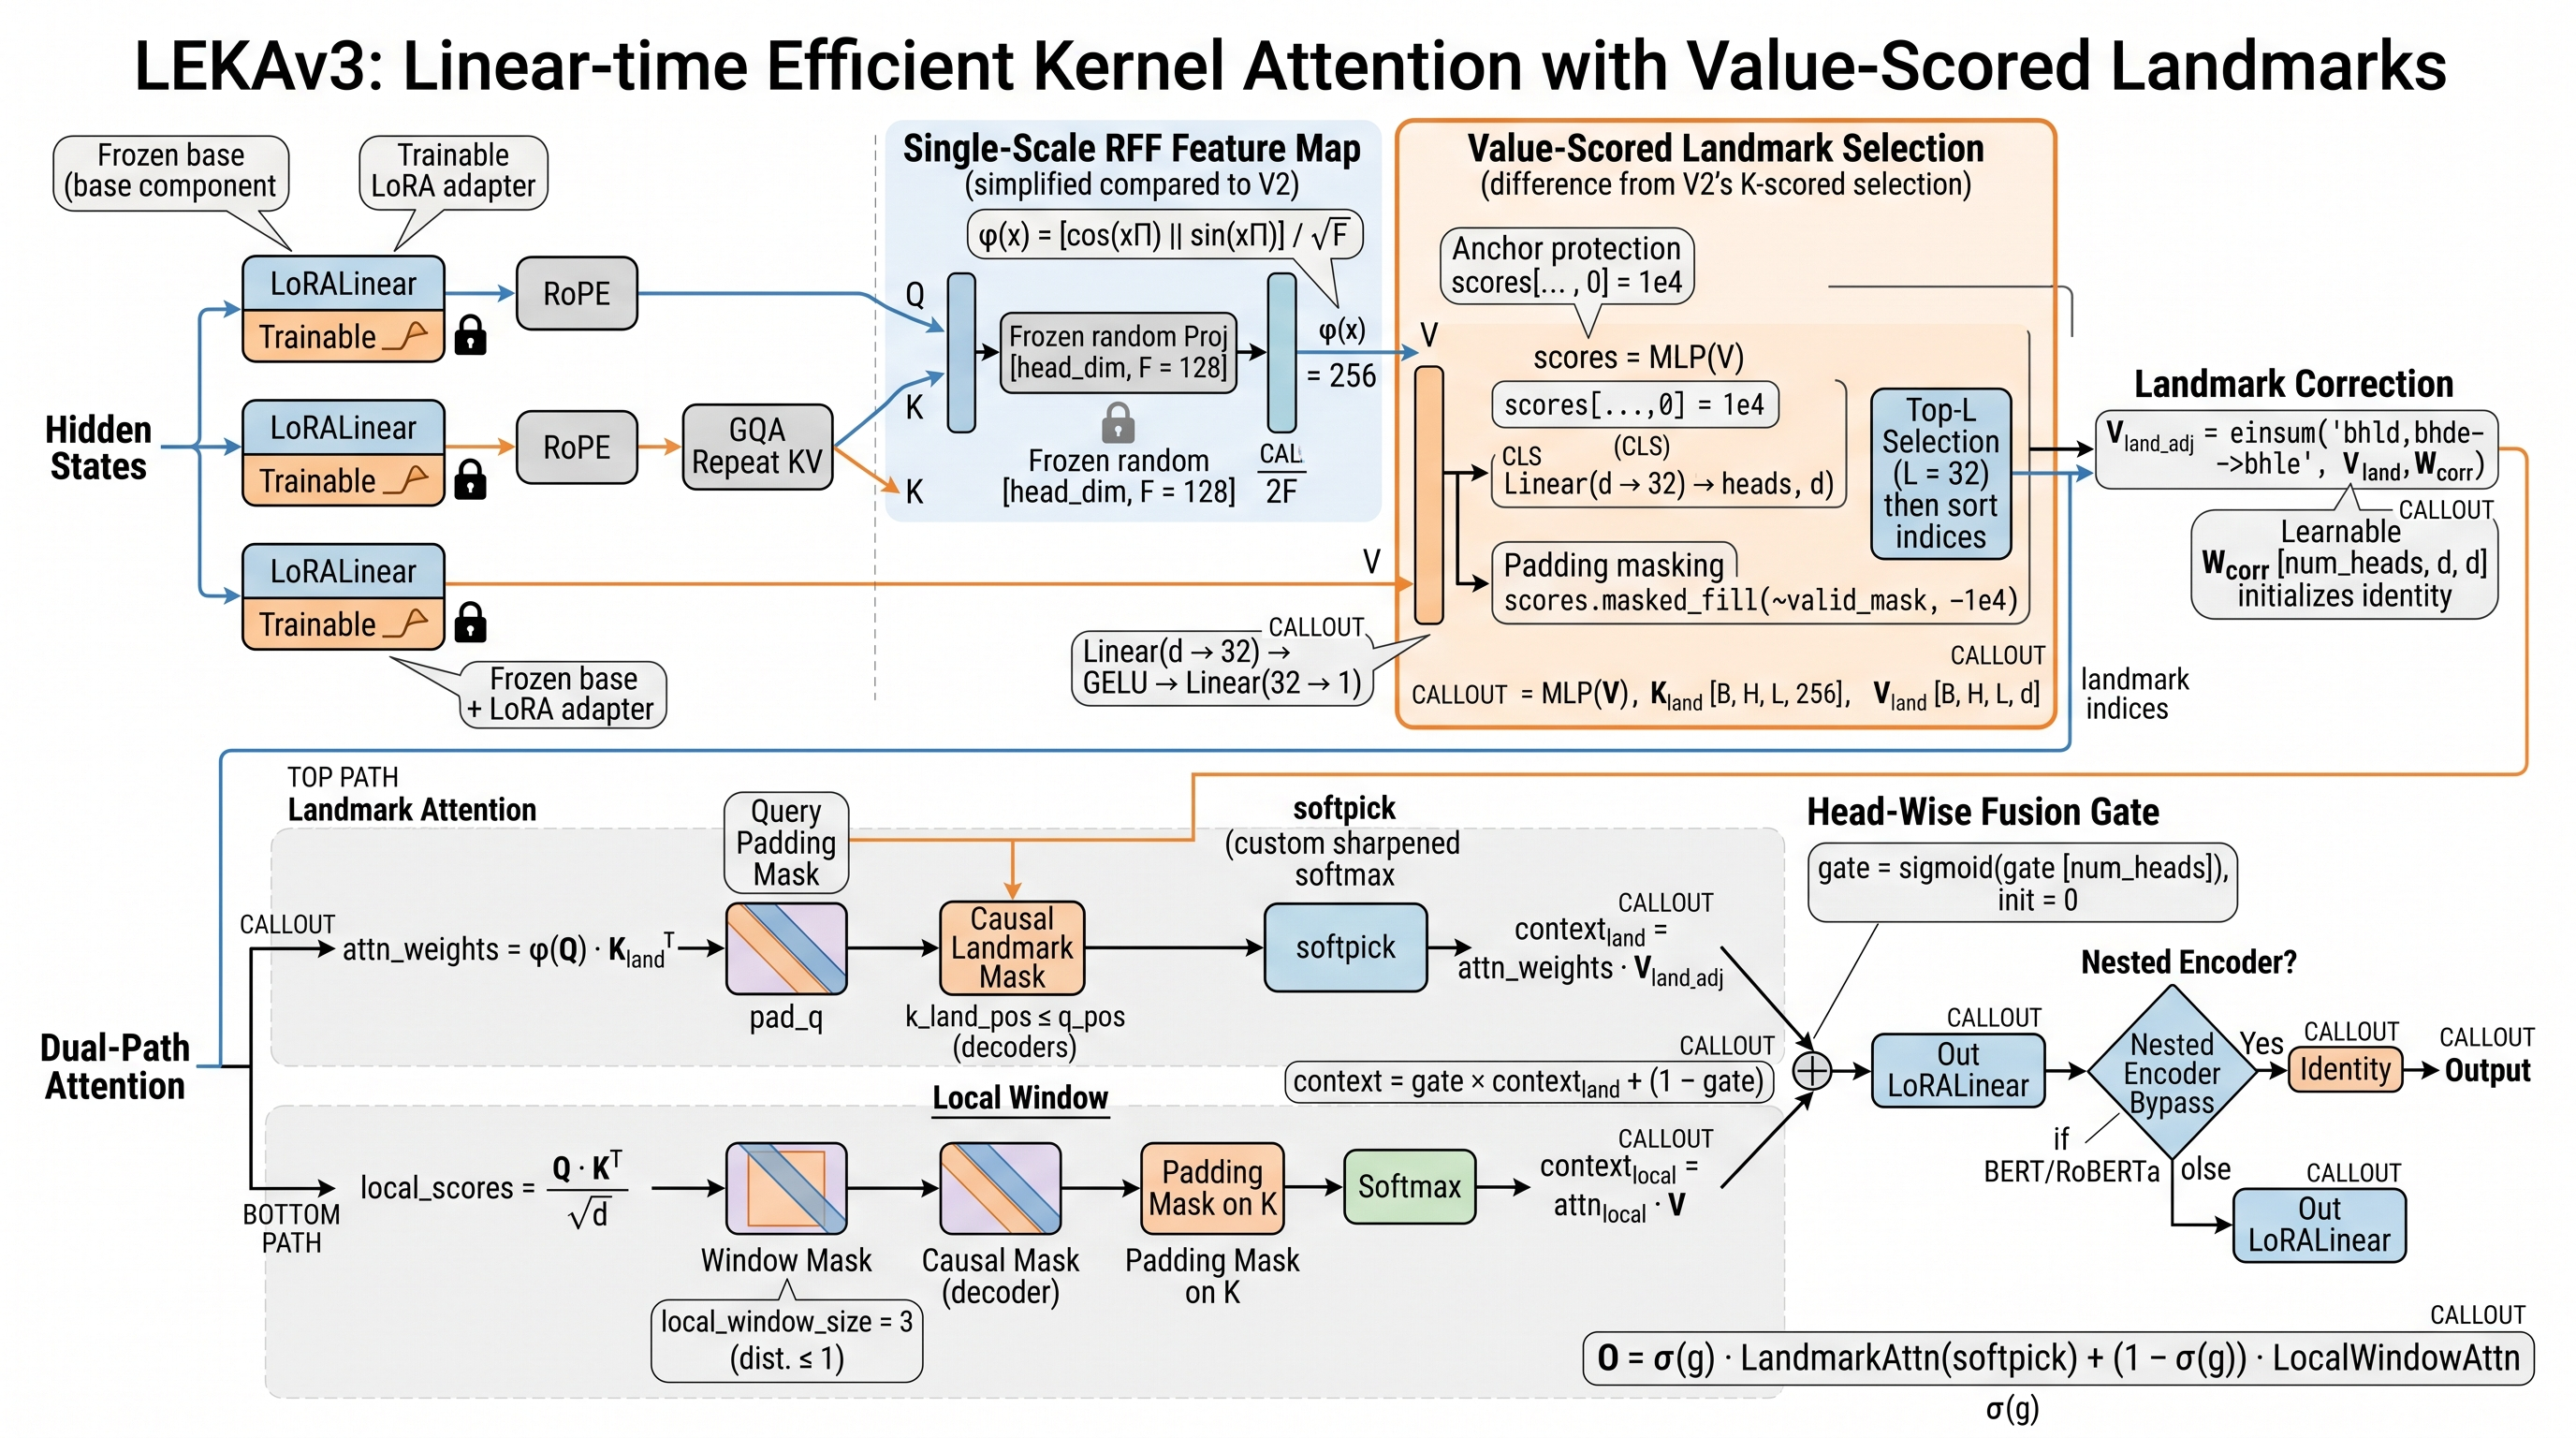
\includegraphics[width=\linewidth]{figures/architecture.jpeg}
\caption{High-level architectural diagram of leka\_v3.}
\label{fig:arch_leka-v3}
\end{figure}

